\documentclass[a4paper,12pt]{article}
\usepackage{graphicx} 
\usepackage{hyperref}
\usepackage{float}

% \begin{figure}[H]
%     \centering
%     \includegraphics[width=0.7\textwidth]{filename.png}
%     \caption{Your figure caption here.}
%     \label{fig:yourlabel}
% \end{figure}

\begin{document}

\title{Assignment 2 \\
YouTube Trending Videos Analysis}
\author{Mohammad Hossein Basouli}
\date{\today}
\maketitle

\begin{center}
    \textit{\section*{Abstract}}
    \textit{In this analysis we will try to uncover hidden relationships and patterns behind a video sharing platform in order to be able to get insights for future decission for 
    growing the related products. We start off by forming different questions about the data, and then through answering these questions grow our understanding of the data. 
    This analysis would lead us to find impactful and correlated factors with some variables like engagement metrics, discover seasonal patterns in trending date and publish date of 
    videos, significane of overall popularity of different video categories on appearance on the top most trending videos and so much more.}
\end{center}

% ---------------------------------------------------------------------------------------------------------------------------------------------------------------------------------------------------------------------- %

\section*{Introduction}
\noindent \textbf{Background}: Analysis of relationships \& and patterns in video streaming and sharing applications has been a matter of great interest since the beginning of development of
these kinda services. It matters so much to be able to answer questions like why some special kind of videos get more views and the others don't, or what factors affects engagement of users 
on different videos and so on. \\

\noindent \textbf{Objectives}: 
\begin{enumerate}
    \item Explaining the data; where it's coming from, an explanation of the features, etc. in \textbf{A Description of the Data} and \textbf{Features} sub sections.
    \item Preprocess the data in order to handle \textit{integration} and \textit{inconsistency} issues in \textbf{Data Preprocessing} sub section. And finally add additional features
    to work with in \textbf{Feature Engineering} sub section.
    \item We will start our analysis in \textbf{Exploratory Data Analysis (EDA)} section by providing different plots of the data and analysing various aspects of it.
    \item After answering our initial questions, it's time to form additional questions about the dataset to gain a broader view of it.
    \item And at the end, we shall summarize our understanding of the data in \textbf{Connecting the Dots} sub section.
\end{enumerate}

\noindent \textbf{Initial Questions}: 
\begin{enumerate}
    \item How are engagement metrics (views, likes and dislikes) distributed overall and across different video categories?
    \item Which YouTube channels and video categories trend the most in each country and globally?
    \item Are there seasonal or day-of-week patterns in trending videos? How does the upload day and time impact video engagement?
    \item Do controversial videos, defined by a high dislike ratio, receive more engagement than universally liked ones?
    \item How do video tags influence engagement, and which tags are most commonly used in trending videos?
    \item How does the length of a video title impact engagement levels?
\end{enumerate} 

% ----------------------------------------------------------------------------------------------------------------------------------------------------------------------------------------------------------------------

\section*{Data}
\subsection*{A Description of the Data}
The dataset has been gathered from the set of trending YouTube videos across 10 different regions in 2 different years (2017/18). The cumulative dataset contains 373,204 rows (trending video records) and 21 columns (features).

\subsection*{Features}
Important numerical features include: \textit{views, likes, dislikes, and comment\_count}. Important categorical and datetime features include: \textit{trending\_date, title (title of the video), 
channel\_title, publish\_time, tags, comments\_disabled, ratings\_disabled, country, category\_title}.

\subsection*{Data Preprocessing}
\noindent \textbf{Handling Missing Values}: The only column that contains missing values is \textit{description} which we shall not use in the course of our analysis. Thus we remove this column along
with other unnecessary columns. \\ 

\noindent \textbf{Duplicated Values}: Since the dataset contains multiple records related to a single video for different \textit{trending dates} in each \textit{country}, we have to be cautious about this 
fact in our future analysis, thus we shall only keep those with the maximum views. Also we must remove the records which have the same \textit{video\_id, country} and \textit{trending\_date} since these records are duplicates. \\

\subsection*{Feature Engineering}
We shall add multiple new features in our dataset in order to capture new information.

\begin{itemize}
    \item Add engagement\_score \& dislike\_rate:
    \( engagement\_score = \frac{likes + dislikes + comment_count}{views} \), \( dislike\_rate = \frac{dislikes}{likes + dislikes} \)
    \item Add day\_of\_trend and season\_of\_trend from trending\_date.
    \item Add season\_of\_publish, day\_of\_publish and hour\_of\_publish from publish\_date.
\end{itemize}
% ----------------------------------------------------------------------------------------------------------------------------------------------------------------------------------------------------------------------

\section*{Exploratory Data Analysis (EDA)}
\subsection*{Visualization}
\noindent \textbf{Distribution of Engagement Metrics}: If we have a look at overall distribution of \textbf{engagement metrics} on Figure~\ref{fig:Figure_1} and their distributions across different \textbf{video categories} on Figure~\ref{fig:Figure_2}, 
we can say that all of the \textbf{engagement metrics} have a long-tail distribution on the right and most of the data are distributed over a very narrow range to the left. And also among different \textbf{video categories}, 
\textit{Music} and \textit{Entertainment} seem to have a higher \textbf{engagement metrics} in general. \\ 

\begin{figure}[H]
    \centering
    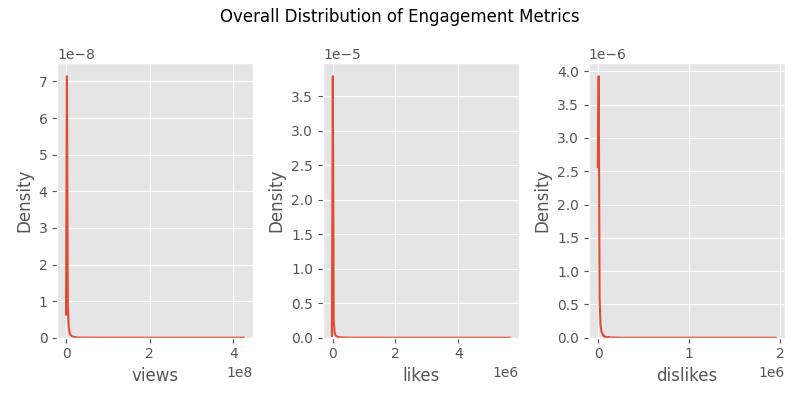
\includegraphics[width=0.7\textwidth]{./images/overall_distro_of_eng_metrics.png}
    \caption{Overall Distribution of Engagement Metrics}
    \label{fig:Figure_1}
\end{figure}

\begin{figure}[H]
    \centering
    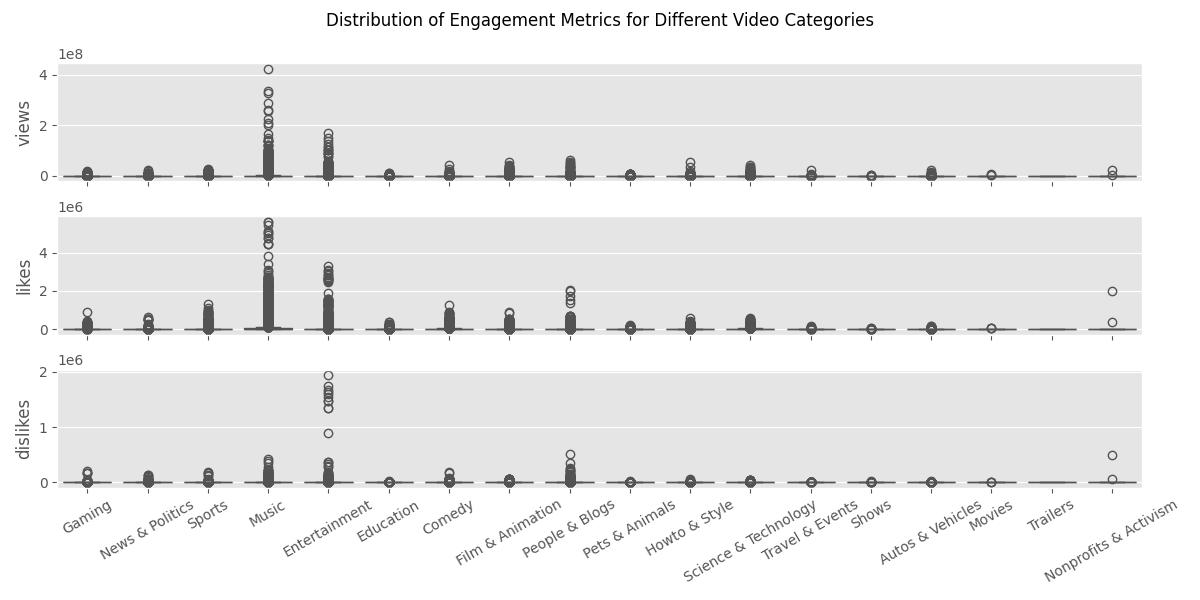
\includegraphics[width=0.7\textwidth]{./images/distro_of_eng_for_diff_cats.png}
    \caption{Distribution of Engagement Metrics Across Different Video Categories}
    \label{fig:Figure_2}
\end{figure}


\noindent \textbf{Effect of Day/Hour of Publish on Engagment Score}: By looking at Figure~\ref{fig:Figure_3}, we don't see a strong relationship between these factors. Thus we shall say that these features 
are independent.

\begin{figure}[H]
    \centering
    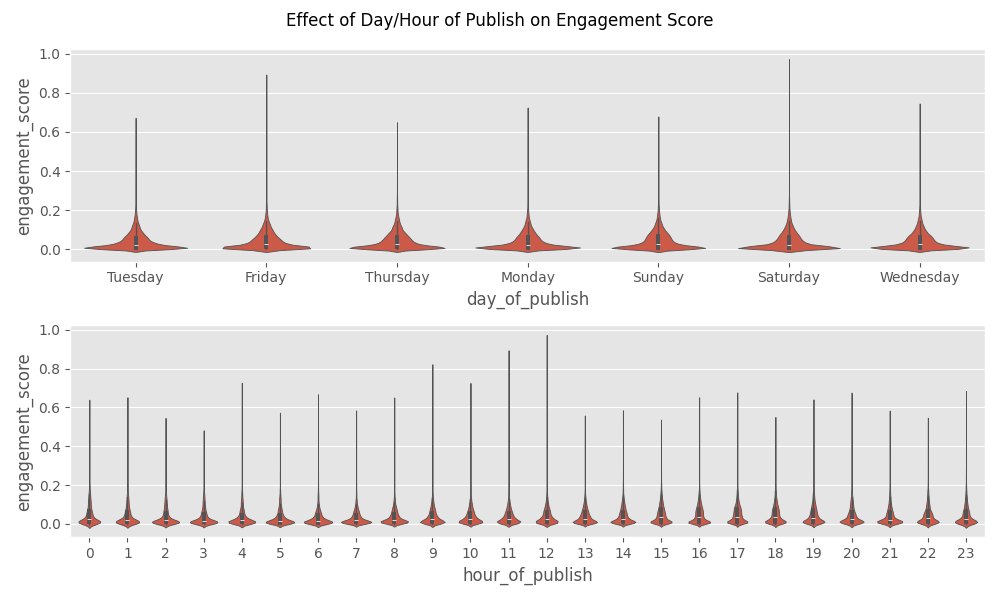
\includegraphics[width=0.7\textwidth]{./images/daily_hourly_pattern_in_eng_score.png}
    \caption{Effect of Day/Hour of Publish on Engagment Score}
    \label{fig:Figure_3}
\end{figure}


\noindent \textbf{Effect of Dislike Ratio on Engagement Score}: If we have a look at Figure~\ref{fig:Figure_4}, we can say that \textit{universally-liked} group has a little higher \textbf{engagement score}. 
But we will investigate this relationship more, later in \textbf{Further Analysis} sub section.

\begin{figure}[H]
    \centering
    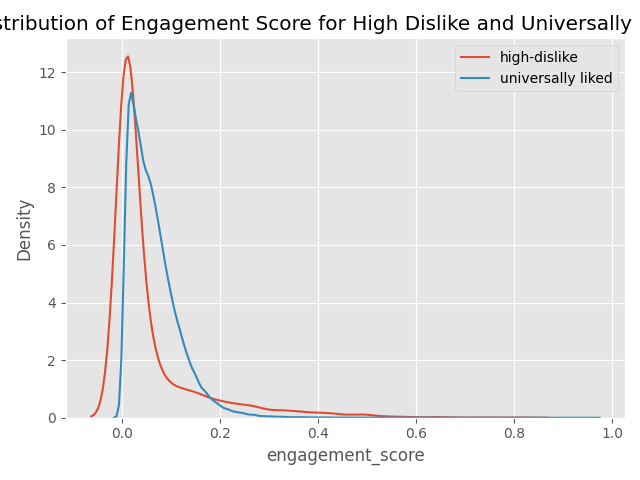
\includegraphics[width=0.7\textwidth]{./images/effect_of_high_dislike_on_eng.png}
    \caption{Effect of Dislike Ratio on Engagement Score}
    \label{fig:Figure_4}
\end{figure}


\noindent \textbf{Relationship between Tag and Engagement Score}: Figure~\ref{fig:Figure_5} tells us that some \textbf{tags} have a better \textbf{engagement score} overally. 
e.g. \textit{review} and \textit{music} have a significatly higher \textbf{engagement\_scores} medians.

\begin{figure}[H]
    \centering
    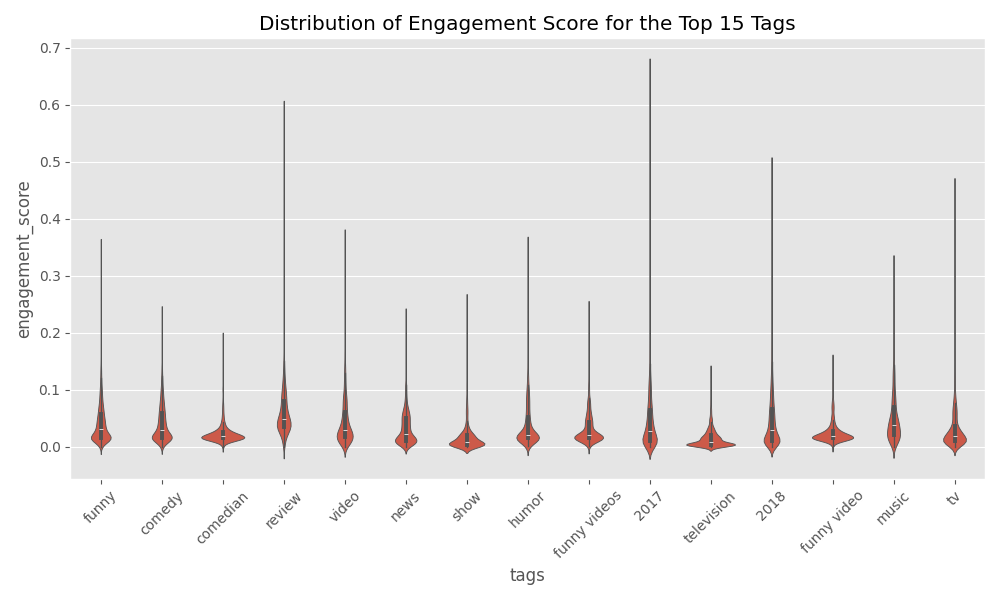
\includegraphics[width=0.7\textwidth]{./images/distro_of_eng_for_top_15_common_tags.png}
    \caption{Relationship between Tag and Engagement Score}
    \label{fig:Figure_5}
\end{figure}


\noindent \textbf{Correlation between Title Length \& Engagement Score}: By looking at Figure~\ref{fig:Figure_6} we can say that, there isn't a strong relationship between these two features.

\begin{figure}[H]
    \centering
    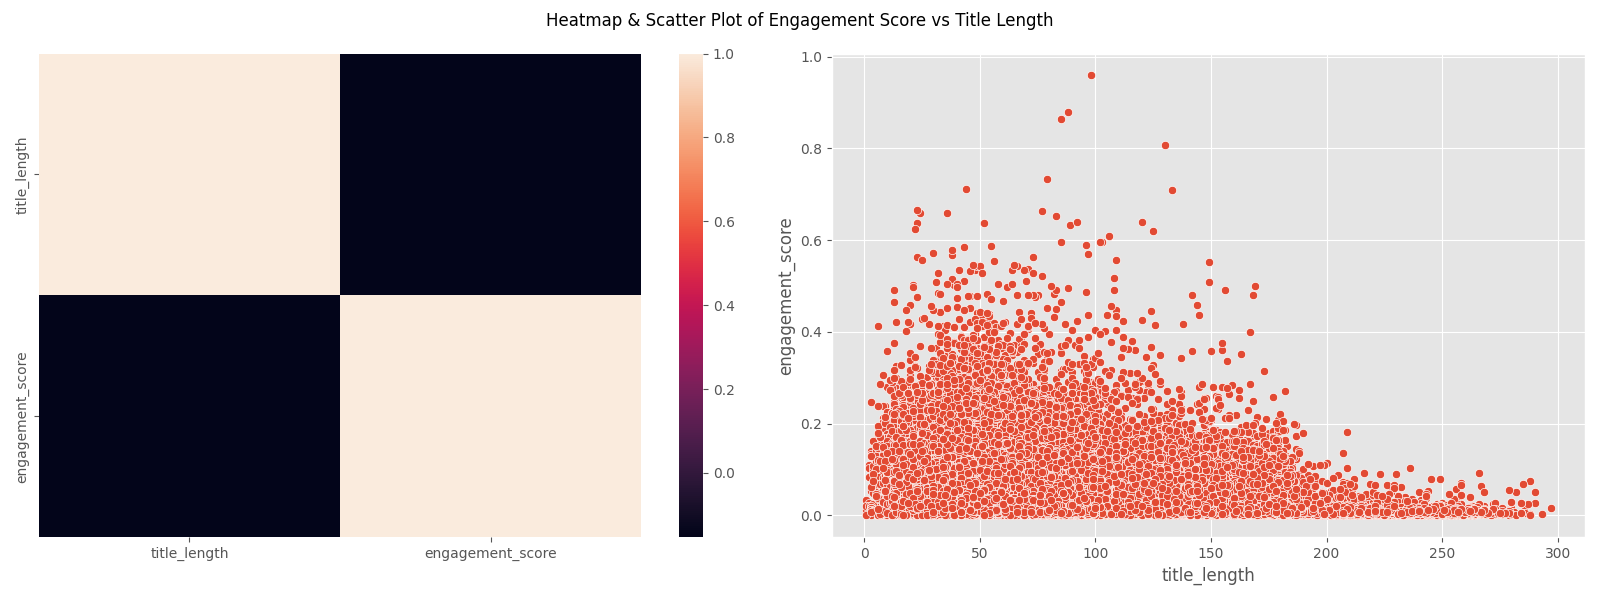
\includegraphics[width=0.7\textwidth]{./images/heatmap_and_scatter_plot_of_eng_vs_title_len.png}
    \caption{Correlation between Title Length \& Engagement Score}
    \label{fig:Figure_6}
\end{figure}


\noindent \textbf{Most Viewed Video, Channel and Video Category across Different Countries and Globally}: If we look at Figure~\ref{fig:Figure_7} we can easily see the most trending \textbf{video}, \textbf{channel} and \textbf{video category} in each country.
Some interesting points worth noting here: 
\begin{itemize}
    \item A single category, channel and video, namely \textit{Entertainment, Youtube Spotlight, Youtube Rewind: The Shape of 2017 | \#YouTubeRewind} has dominated the most viewed \textbf{categories}, 
    \textbf{channels} and \textbf{videos} by appearing in six regions!
    \item Only two \textbf{videos categories} appear in this list, meaning that most viewed videos in different regions have most likely the same \textbf{video category}.
    \item A single video stands as the most trending video in six different \textit{regions}.
\end{itemize}

\begin{figure}[H]
    \centering
    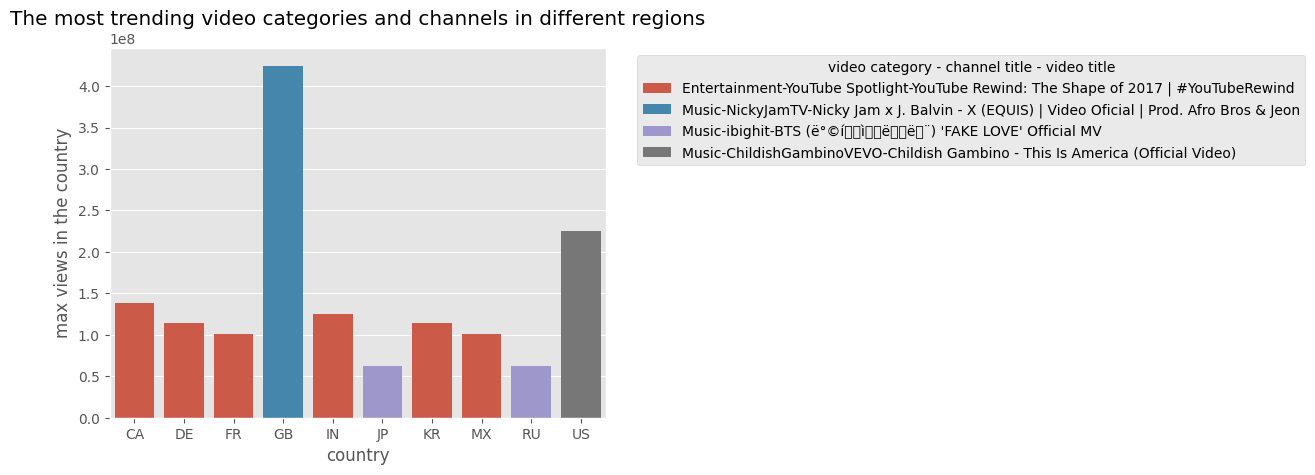
\includegraphics[width=0.7\textwidth]{./images/most_trend_cats_and_chanells_diff_regions.png}
    \caption{Most Viewed Video, Channel and Video Category across Different Countries and Globally}
    \label{fig:Figure_7}
\end{figure}


\noindent \textbf{Seasonal/Daily Patterns in Trending Date}: Figure~\ref{fig:Figure_8} shows that we have a significant difference in the number of trending videos in each season. e.g. \textit{Spring} and \textit{Winter} 
have so many more trending videos in them. 

\begin{figure}[H]
    \centering
    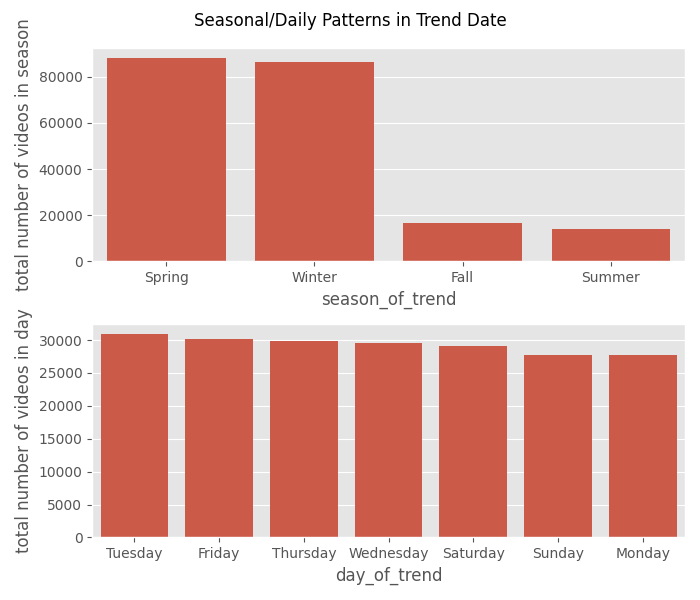
\includegraphics[width=0.7\textwidth]{./images/seasonal_daily_patterns_in_trend_date.png}
    \caption{Seasonal/Daily Patterns in Trending Date}
    \label{fig:Figure_8}
\end{figure}


\noindent \textbf{Top 10 Tags}: Figure~\ref{fig:Figure_9} shows the top 10 \textbf{tags} and their number of occurances.

\begin{figure}[H]
    \centering
    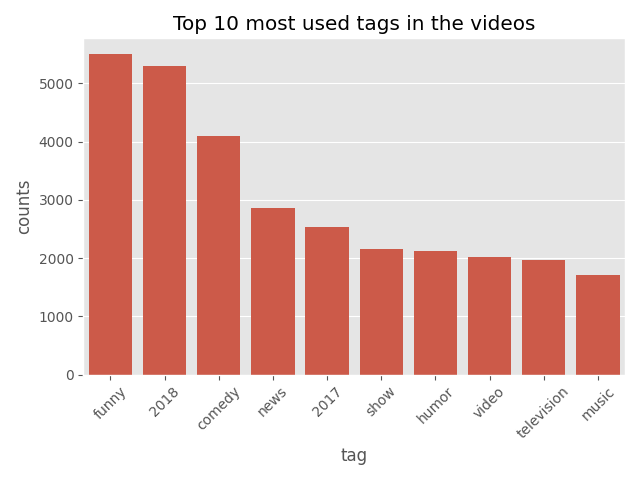
\includegraphics[width=0.7\textwidth]{./images/top_ten_most_used_tags.png}
    \caption{Top 10 Tags}
    \label{fig:Figure_9}
\end{figure}


\subsection*{Furthur Analysis} 
Now we want to investiagte the dataset more to gain more insights. \\

\noindent \textbf{Frequency Distribution of the Video Categories}: If we have a look at Figure~\ref{fig:Figure_10} we can observe each of the categories along with their frequency percentages.

\begin{figure}[H]
    \centering
    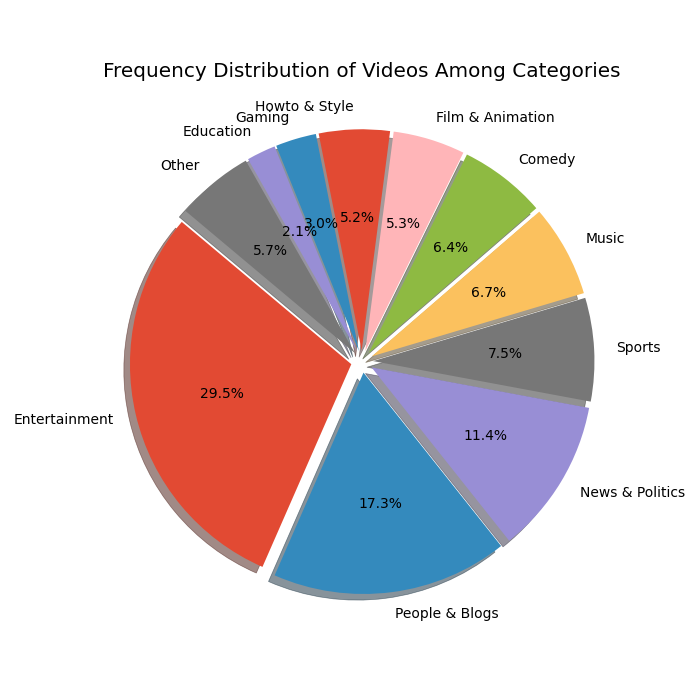
\includegraphics[width=0.7\textwidth]{./images/frequency_distribution_of_videos_among_categories.png}
    \caption{Frequency Distribution of the Different Video Categories}
    \label{fig:Figure_10}
\end{figure}


\noindent \textbf{Top 5 Most Trending Categories per Each Year}: By looking at Figure~\ref{fig:Figure_11} we find out that there has been a huge increase in the number of usages for some 
categories such as \textit{Entertainment, People \& Blogs and News \& Politics etc.}. Also we find out that \textit{Music} has not been of great interest in the year 2017 but has been replaced 
with \textit{Comedy} category in the year 2018.

\begin{figure}[H]
    \centering
    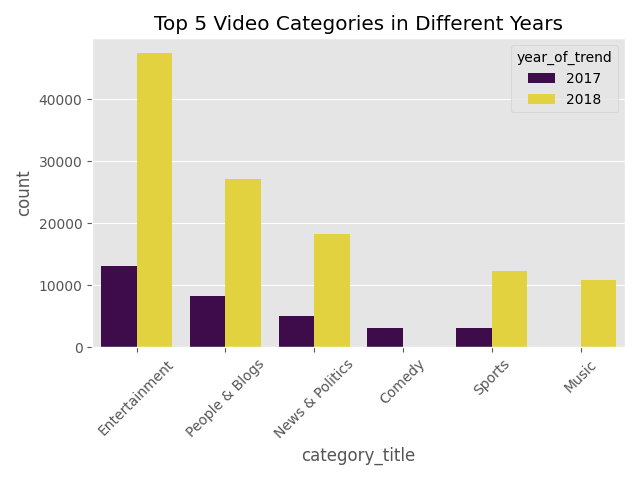
\includegraphics[width=0.7\textwidth]{./images/top_5_video_categories_in_diff_years.png}
    \caption{Top 5 Categories in Each Year}
    \label{fig:Figure_11}
\end{figure}


\noindent \textbf{Seasonal/Daily Pattterns in Publish Time}: Figure~\ref{fig:Figure_12} shows us a significant difference across different \textbf{seasons} in the number of \textbf{publishes}. e.g. \textit{Spring} and \textit{Winter} have 
many more \textit{publishes} compared to other \textbf{seasons}. But there isn't that much of difference in different \textbf{days of week} in terms of \textbf{number of publishes} 

\begin{figure}[H]
    \centering
    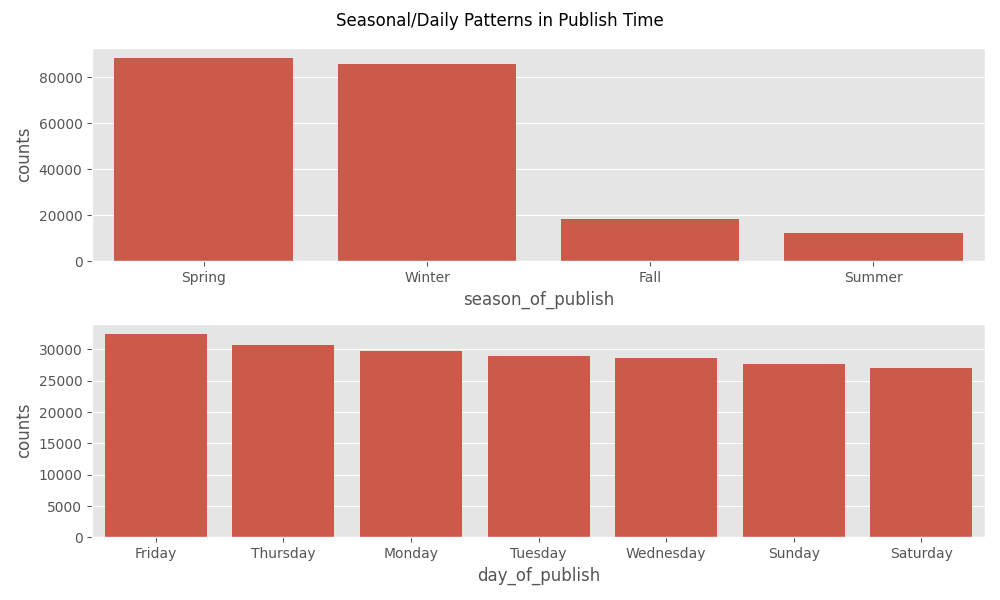
\includegraphics[width=0.7\textwidth]{./images/seasonal_daily_patterns_in_publish_time.png}
    \caption{Seasonal/Daily Patterns in Publish Time}
    \label{fig:Figure_12}
\end{figure}


\noindent \textbf{Effect of Comments Being Disabled on Likes}: If we have a look at Figure~\ref{fig:Figure_13}, we can say that there is a significant difference between these two groups of data. Meaning that 
video with \textit{comments enabled} get more \textbf{likes} in general.

\begin{figure}[H]
    \centering
    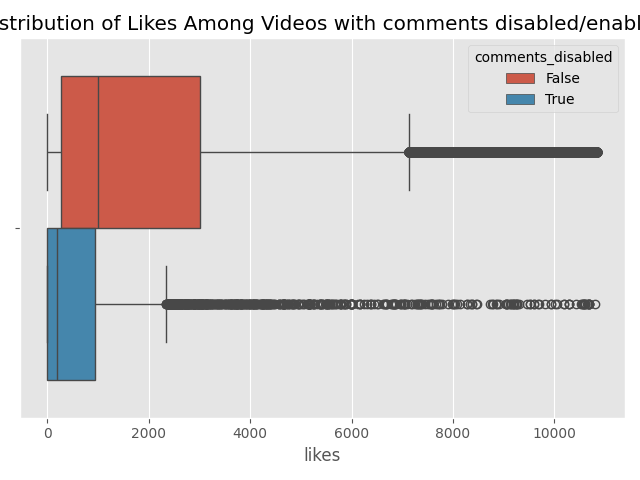
\includegraphics[width=0.7\textwidth]{./images/distro_of_likes_among_vids_with_cmnt_dis_enb.png}
    \caption{Effect of Comments Being Disabled on Likes}
    \label{fig:Figure_13}
\end{figure}


\noindent \textbf{Top 10 Categories in Having Videos with Comments Disabled}: By having a look at Figure~\ref{fig:Figure_14}, we see that the \textbf{categories} \textit{Entertainment, News \& Politics, Education and Film \& Animation} 
have took the lead in terms of having more videos with \textit{comments disabled}. It's is really interesting to see this huge amount of videos with \textit{comments disabled} in \textit{News \& Politics} \textbf{category}.  

\begin{figure}[H]
    \centering
    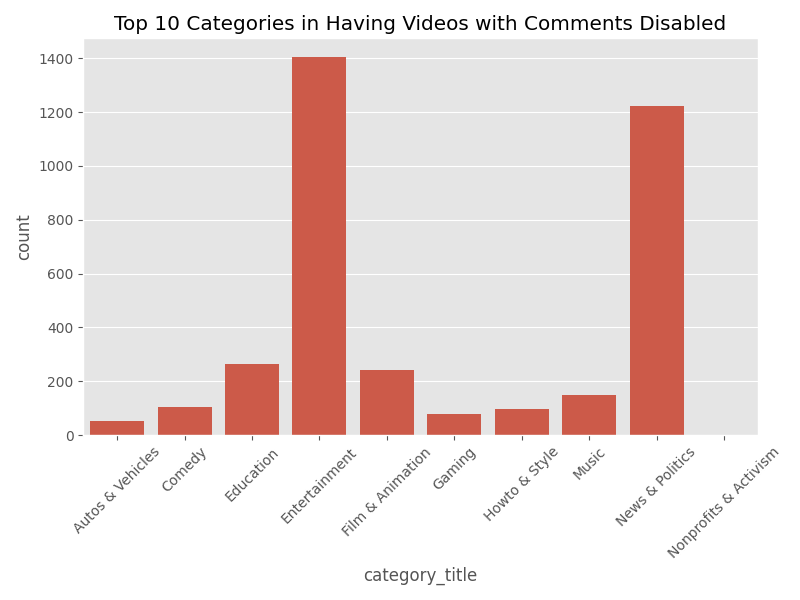
\includegraphics[width=0.7\textwidth]{./images/distribution_of_dis_cmnt_diff_cat.png}
    \caption{Top 10 Categories in Having Videos with Comments Disabled}
    \label{fig:Figure_14}
\end{figure}


\noindent \textbf{Effect of Dislike Ratio on Views}: Figure~\ref{fig:Figure_15} shows that as we move from \textit{low} \textbf{dislike ratios} to \textit{higher} \textbf{dislikes ratios}, we will find fewer and fewer videos with an extremely high 
amount of views, meaning that videos with extremely high amount of views have at least a moderately good like ratio.

\begin{figure}[H]
    \centering
    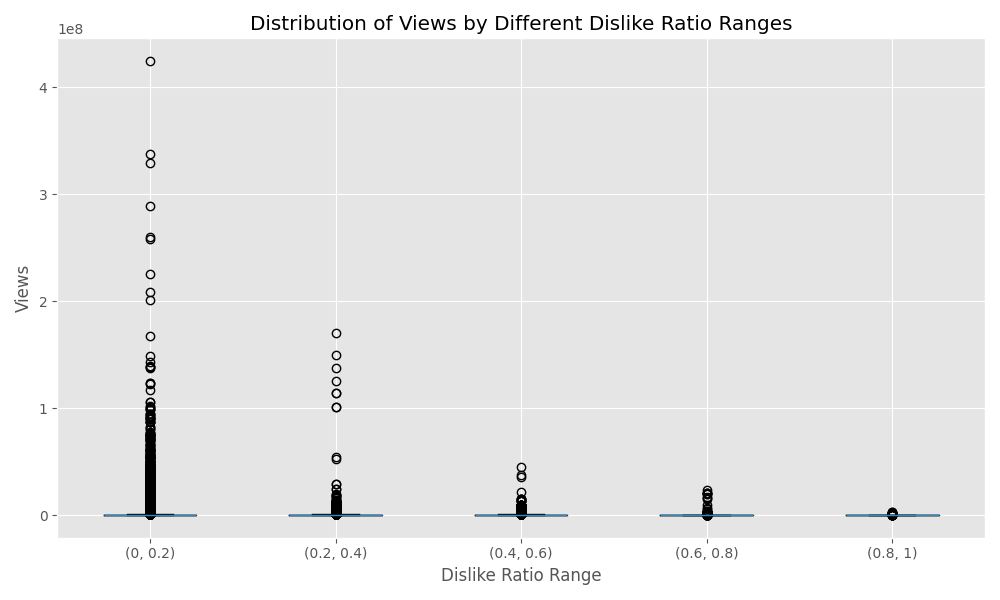
\includegraphics[width=0.7\textwidth]{./images/distro_of_views_diff_dis_ratio_ranges.png}
    \caption{Effect of Dislike Ratio on Views}
    \label{fig:Figure_15}
\end{figure}


\noindent \textbf{Effect of Dislike Ratio on Engagement Score}: By looking at Figure~\ref{fig:Figure_16} we can see a nice pattern unraveling. We observe that videos with extremely low or high dislike ratio are in a slightly better 
situation in terms of \textbf{engagement score} comapred to the videos with a more moderate dislike ratio.   

\begin{figure}[H]
    \centering
    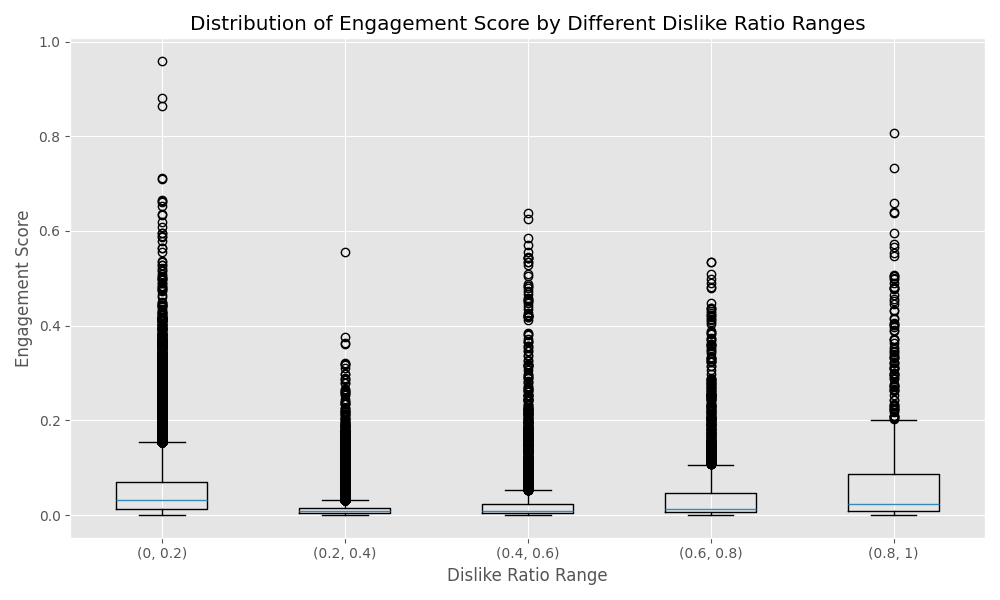
\includegraphics[width=0.7\textwidth]{./images/distro_of_eng_score_diff_dis_ratio_ranges.png}
    \caption{Effect of Dislike Ratio on Engagement Score}
    \label{fig:Figure_16}
\end{figure}


\subsection*{Connecting the Dots}
Now we will try to connect the insights that we have taken from our analysis and combine them to deepen our understanding of the relationships and patterns that exists in the data. \\ 

\noindent \textbf{Infuental Factors for Engagement Score}: Based on the prior analysis on Figure~\ref{fig:Figure_16}, Figure~\ref{fig:Figure_5}, Figure~\ref{fig:Figure_4} and Figure~\ref{fig:Figure_9},  we find out that 
the variables \textbf{dislike ratio} and \textbf{tags} have significant impacts on the variable \textbf{engagement score}. For exmple very high or very low \textbf{dislike ratios} comes with 
more \textbf{engagement scores} as well. Or videos with some certain \textbf{tags} like \textit{review} and \textit{music} appear in videos which have higher engagement scores in general, 
whereas some others like \textit{television, show} and \textit{comedian}. Also it worth mentioning that frequency of occurance of a tag doesn't mean that it will gain higher \textbf{engagement scores}. e.g. the \textbf{tags} \textit{funny, 2018, comedy, news} 
and \textit{2017} despite of being at the top of most used \textit{tags} list, have a moderate \textbf{engagement score} in general. \\

\noindent \textbf{Difference of Development in Different Categories and Hidden Impact of Each on Videos Being Trended}: From our earlier analysis on Figure~\ref{fig:Figure_7}, Figure~\ref{fig:Figure_10} and Figure~\ref{fig:Figure_11}, we can say 
that some categories have been developed so much more than the others over the course of these two year (2017-18); e.g. \textit{Entertainment} has got 4 times more popular, 
\textit{People \& Blogs} has got 3 times more popular, whereas \textit{Comedy} has been kicked out of the list. And also despite \textit{Music} tag has been placed at 5-th place in terms of total occurances, 
it stands as the category of most trended video in one thirds of the regions, meaning that this category appears on few videos but it only appears on the most trending ones. \\

\noindent \textbf{Infuental Factors in Engagement Metrics}: From what was saw in our prior analysis on Figure~\ref{fig:Figure_2}, Figure~\ref{fig:Figure_13} and Figure~\ref{fig:Figure_15}, we find out 
that some influential factors on \textbf{engagement metrics} are \textbf{dislike ratio}, \textbf{comments being enabled/disabled for the video} and \textbf{video category}. e.g. The \textbf{video categories} \textit{Music} and \textit{Entertainment} are the two 
have higher values \textbf{engagement metrics} in general. Or videos with \textbf{comments being enabled} receive higher amounts of \textbf{like} in general compared to those which have it turned off. 
or as the \textbf{dislike ratio} of a video increases, its likelihood of having a very large amoung of views decreases dramatically. \\ 

\noindent \textbf{Similar Seasonal Pattern in Trending Date and Publish Date}: If we turn back to the analysis that we have done on Figure~\ref{fig:Figure_8} and Figure~\ref{fig:Figure_12} we can 
see that there is a very similar \textit{seasonal} pattern between \textbf{trending date} and \textbf{publish date}. Both of these variables seem to happen often on the same \textit{seasons} more often. \\ 
 
\noindent \textbf{Special Categories Are Not Open to Discussions}: By looking back at our analysis on Figure~\ref{fig:Figure_14}, we can bring more insights on the table. e.g. 
the videos in the \textbf{category} \textit{News \& Politics} don't want to hear comments and have discussions about their videos whereas almost none of the videos in the \textbf{category} 
\textit{Nonprofits \& Activism} have their comments disabled and want to hear about users' comments and concerns about the video. \\ 

% ----------------------------------------------------------------------------------------------------------------------------------------------------------------------------------------------------------------------

% Hypothesis Testing %

% ----------------------------------------------------------------------------------------------------------------------------------------------------------------------------------------------------------------------

% Conclusion %

% ----------------------------------------------------------------------------------------------------------------------------------------------------------------------------------------------------------------------

% Decission Making %

\end{document}